\begin{song}{title=\centering House Of The Rising Sun \\\normalsize \vspace*{-0.3cm}}  %% sem se napíše jméno songu a autor
\moveright \stred \vbox{      %Varianta č. 1  ---> Jeden sloupec zarovnaný na střed	

\sloka 
	^{Ami\,}There is a ^{C{\color{white}\_\_}}house in ^{D{\color{white}\_}}New ^{F}Orleans
	
	they ^{Ami}call the ^{C{\color{white}\_\_}}Rising ^{E}Sun

	and it's ^{Ami}been a ^{C}ruin of ^{D}many a poor ^{F}boy

	and ^{Ami}God I ^{E}know I'm ^{Ami}one. ^{C\,D\,F\,Ami\,E\,Ami\,E}

\sloka
	My mother was a tailor
	
	sewed my new blue jeans,
	
	my father was a gamblin' man
   	
   	down in New Orleans.

\sloka
	Now the only thing a gambler needs
   	
   	is suitcase and trunk
   	
   	and the only time he's satisfied
   	
   	is when he's on, a drunk.

\sloka
	Oh mother tell your children
   	
   	not to do what I have done
   	
   	spend your lives in sin and misery
	
	in the House of the Rising Sun.

\sloka
	Well, I've got one foot on the platform
   	
   	the other foot on the train
   	
   	I'm going back to New Orleans
   	
   	to wear that ball and chain.

\sloka = 1.



}
\setcounter{Slokočet}{0}
\end{song}

\begin{figure}[h]
\centering

\includegraphics[scale=1.5]{../Akordy/am.png}
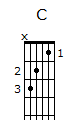
\includegraphics[scale=1.5]{../Akordy/c.png}

\includegraphics[scale=1.5]{../Akordy/d.png}

\includegraphics[scale=1.5]{../Akordy/f.png}
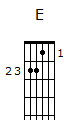
\includegraphics[scale=1.5]{../Akordy/e.png}
\end{figure}

